% Options for packages loaded elsewhere
\PassOptionsToPackage{unicode}{hyperref}
\PassOptionsToPackage{hyphens}{url}
%
\documentclass[
]{article}
\usepackage{lmodern}
\usepackage{amssymb,amsmath}
\usepackage{ifxetex,ifluatex}
\ifnum 0\ifxetex 1\fi\ifluatex 1\fi=0 % if pdftex
  \usepackage[T1]{fontenc}
  \usepackage[utf8]{inputenc}
  \usepackage{textcomp} % provide euro and other symbols
\else % if luatex or xetex
  \usepackage{unicode-math}
  \defaultfontfeatures{Scale=MatchLowercase}
  \defaultfontfeatures[\rmfamily]{Ligatures=TeX,Scale=1}
\fi
% Use upquote if available, for straight quotes in verbatim environments
\IfFileExists{upquote.sty}{\usepackage{upquote}}{}
\IfFileExists{microtype.sty}{% use microtype if available
  \usepackage[]{microtype}
  \UseMicrotypeSet[protrusion]{basicmath} % disable protrusion for tt fonts
}{}
\makeatletter
\@ifundefined{KOMAClassName}{% if non-KOMA class
  \IfFileExists{parskip.sty}{%
    \usepackage{parskip}
  }{% else
    \setlength{\parindent}{0pt}
    \setlength{\parskip}{6pt plus 2pt minus 1pt}}
}{% if KOMA class
  \KOMAoptions{parskip=half}}
\makeatother
\usepackage{xcolor}
\IfFileExists{xurl.sty}{\usepackage{xurl}}{} % add URL line breaks if available
\IfFileExists{bookmark.sty}{\usepackage{bookmark}}{\usepackage{hyperref}}
\hypersetup{
  pdftitle={Untitled},
  hidelinks,
  pdfcreator={LaTeX via pandoc}}
\urlstyle{same} % disable monospaced font for URLs
\usepackage[margin=1in]{geometry}
\usepackage{graphicx,grffile}
\makeatletter
\def\maxwidth{\ifdim\Gin@nat@width>\linewidth\linewidth\else\Gin@nat@width\fi}
\def\maxheight{\ifdim\Gin@nat@height>\textheight\textheight\else\Gin@nat@height\fi}
\makeatother
% Scale images if necessary, so that they will not overflow the page
% margins by default, and it is still possible to overwrite the defaults
% using explicit options in \includegraphics[width, height, ...]{}
\setkeys{Gin}{width=\maxwidth,height=\maxheight,keepaspectratio}
% Set default figure placement to htbp
\makeatletter
\def\fps@figure{htbp}
\makeatother
\setlength{\emergencystretch}{3em} % prevent overfull lines
\providecommand{\tightlist}{%
  \setlength{\itemsep}{0pt}\setlength{\parskip}{0pt}}
\setcounter{secnumdepth}{-\maxdimen} % remove section numbering

\title{Untitled}
\author{}
\date{\vspace{-2.5em}}

\begin{document}
\maketitle

\hypertarget{CI}{%
\section{Parameter Intervals}\label{CI}}

The \textbf{objective} of this first section is to provide simple
examples of \textbf{reverse engineering} that show some of the logic
behind statistical `confidence intervals' for parameters. We begin with
`100\% confidence' intervals, and then, in section 2, we explain why we
have to move to `less-than-100\% confidence' intervals, where things get
a bit more nuanced. In both sections, we emphasize the reverse
engineering, i.e, by using as our limits the worst-case or
almost-worst-case scenarios involving the (unknown) values of the
parameter that is being estimated.

\hypertarget{confidence-intervals}{%
\subsection{`100\% confidence' intervals}\label{confidence-intervals}}

\textbf{Example 1}

Consider a very `particularistic' parameter, the height of a particular
building. There is nothing `scientific' about the parameter, except
maybe that we use tools of mathematical science (of trignometry) to
measure it. Nevertheless, we will sometimes refer to it one of the
generic symbols for a parameter, namely \(\theta.\)

Suppose you measure the height of this building by standing a known
horizontal distance (e.g.~100 metres) from the bottom of the building
and using an instrument to measure the angle between the horizontal and
the top of the building. Suppose, as shown in the left panel of the
Figure below, that the instrument gives a reading of 70 degrees.

Remembering from trigonometry that the tangent of a 70 degree angles is
2.75, the angle of 70 degrees suggests that the height of the building
is \(\hat{\theta}\) = 275 metres. The `hat' is statistical shorthand for
`estimate of.' Since it is sometimes referred to as a `point estimate'
of \(\theta\), we display the value using a dot or point.

After calculating this, you learn that the measuring instrument only
displays the angle is to the nearest 10 degrees. This means that the
true angle is somewhere between 65 and 75 degrees. {[}This is the same
range you would get if it was dark and you used a laser pointer or
flashlight attached to a wheel that rotates in fixed 10-degree steps,
i.e., 5 degrees, 15 degrees, 25 degrees, etc. At 65 degrees, the light
is visible on the building, but at 75 degrees, it goes above the
building and shines into the sky.{]}

So you \textbf{cannot say} that the true height is \textbf{exactly} 275
metres. What \textbf{can} you say? And with what certainty?

You can put \textbf{limits} on the true height by asking \textbf{what
are the minimum and maximum heights that could have produced the
observed reading of 70 degrees?}

To do this you need to take the limits one at a time. The
\textbf{minimum} angle that could have given the (rounded) readout of 70
degrees is 65 degrees, and this corresponds to a minimum height (lower
limit) height of \(\theta_L\) = 214 metres. The \textbf{maximum} angle
that could have given the readout of 70 degrees is 75 degrees, and this
corresponds to a maximum height (upper limit) of \(\theta_U\) = 373
metres. Thus, assuming that the instrument is measuring the angle
correctly, and then doing what you are told it does, you are 100\%
confident that the true height lies in the interval (214, 373). As is
clear in the graph, this does not have the typical 275 \(\pm\) a
single-number (or in sybols, \(\hat{\theta} \pm\) ME {[}`margin of
error'{]}) that we typically see in reports.

\begin{figure}

{\centering 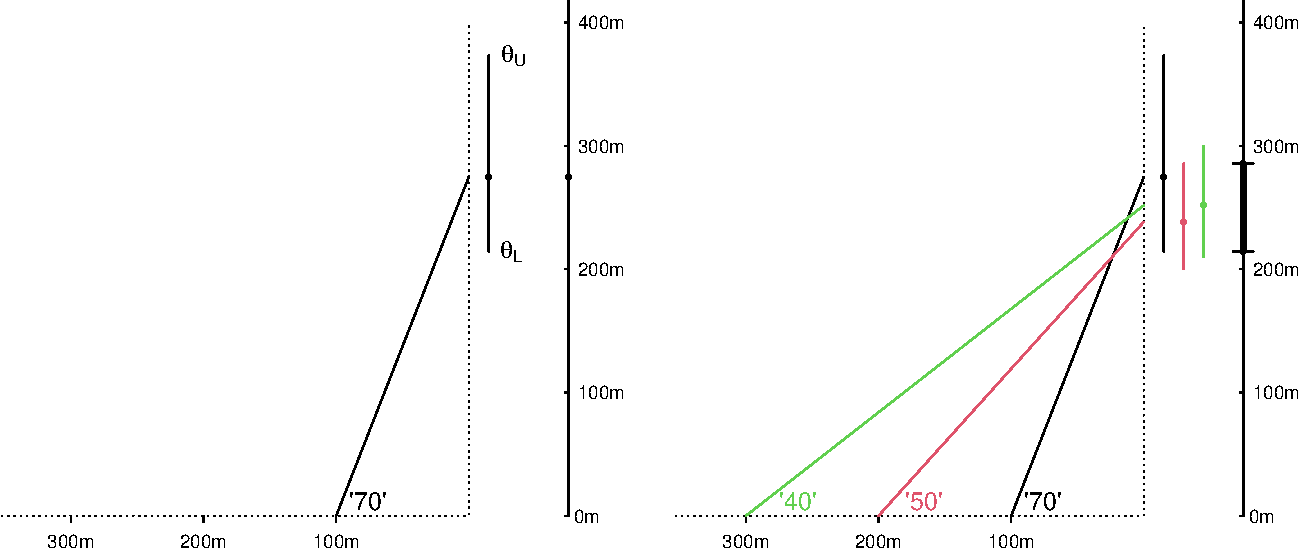
\includegraphics{hanley-ci_files/figure-latex/unnamed-chunk-1-1} 

}

\caption{Estimating the height of an building by measuring subtended angles. The '70' in the left panel signifies that the real angle was somewhere between 65 and 75 degrees; thus the real height lies between the L and U limits of 214 and 373 metres. In the righ panel, the  interval shown by the thicker black segment to the right of the 3 individual intervals is the  set of parameter values common to all 3.}\label{fig:unnamed-chunk-1}
\end{figure}

\textbf{\emph{More data}}

The panel on the right shows how, by obtaining 3 measurements at 3
different distances, and finding the interval they have in common (the
overlap), you can narrow the interval within which the true height must
lie.

\textbf{What allows us to be 100\% confident in the parameter interval}

The reason is the limited error range. How wide the error range is, and
how many measurements one makes, determine how wide the parameter
interval is.

\textbf{Example 2}

This one is less artificial, and indeed is motivated by a real court
case in the late 1990s in Quebec, where a defendant's age (which would
determine wheter he was tried in an adult or a juvenile court) was in
doubt. He was adopted, while still a young child, from another country.
Official birth records were not available, and his adoptive parents were
able to get a cheaper airfare by claiming that he was under age 2 at the
time. Bone age, and Tanner Staging, also known as Sexual Maturity Rating
(SMR), an objective classification system used to track the development
and sequence of secondary sex characteristics of children during
puberty, were other pieces of information used by the judge.

For more on this topic of determining chronological age, see this
article, entitled
\href{https://discovery.ucl.ac.uk/id/eprint/1470308/1/Tim_Cole_Intl_Innovation_140_Research_Media.pdf}{Many
applications for medical statistics} and thos one, entitled
\href{https://rss.onlinelibrary.wiley.com/doi/full/10.1111/j.1740-9713.2012.00568.x}{People
smugglers, statistics and bone age}, by UCL statistics professor and
child growth expert,
\href{https://scholar.google.com/citations?user=1P_yQocAAAAJ\&hl=en}{Tim
Cole}.

Again, the person's correct chronological age is a particularistic
parameter, one that had nothing to do with science, or universal laws of
Nature. But it can be estimated by using the laws of mathematics and
statistics.

For didactic purposes, we will simplify matters, and assume that `our'
indirect method gives estimates such that if many of them were averaged,
they would give the correct chronological age of the person (in
statistical lingo, statisticians say that the method/estimator is
`unbiased'). However, as is seen below, the individual measurements vary
quite a bit around the correct age. They can be off by as much as 25\%
(1/4th) in either direction. {[}In practice, a measuring instrument with
this much measurement error would not be useful -- unless it was fast,
safe, inexpensive, non-invasive, easily repetaed, and so on -- but we
make the measurement variations this large just so we can see the
patters more clearly on the graph!{]}. Another unrealistic feature of
our `measurement model' is that the `error distribution' has a
\textbf{finite range}. The \textbf{shape} of the error distribution
doesn't come into the 100\% `confidence intervals' below, but it will
matter a little bit -- but not a whole lot unless the sample size is
small -- later on when we cut corners.

Consider first a single indirect measurement of chronological age, that
yielded a value of 17.6 years.

Given what you know about the sizes of the possible errors, you
\textbf{cannot say} that the true age is \textbf{exactly} 17.6 years
What \textbf{can} you say? And with what certainty?

You can put \textbf{limits} on the true age by asking \textbf{what are
the minimum and maximum ages that could have produced the observed
reading of} 17.6 years.

To do this you need to consider the limits \textbf{one scenario at a
time}. The \textbf{minimum} age that could have given the estimate of
17.6 years is / 1.125 = 15.7 years. The \textbf{maximum} age that could
have produced this reading is 17.6 / 0.875 = 20.1 years. Thus (assuming
the error model is correct!) you are 100\% confident that the true age
lies in the interval (15.7 , 20.1) years. Again, as is clear in the
graph, this does not have the typical 17.6 \(\pm\) a single-number
margin of error that we typically see in reports. Rather, it is 17.6
\textbf{- 2.6} and 17.6 \textbf{+ 4.4} !

But, you can't arrive at these directly; get there this way. You have to
try on various limits, until

\[ LowerLimit + margin  = 17.6 \ = \   UpperLimit - margin  \]

\textbackslash begin\{figure\}

\{\centering 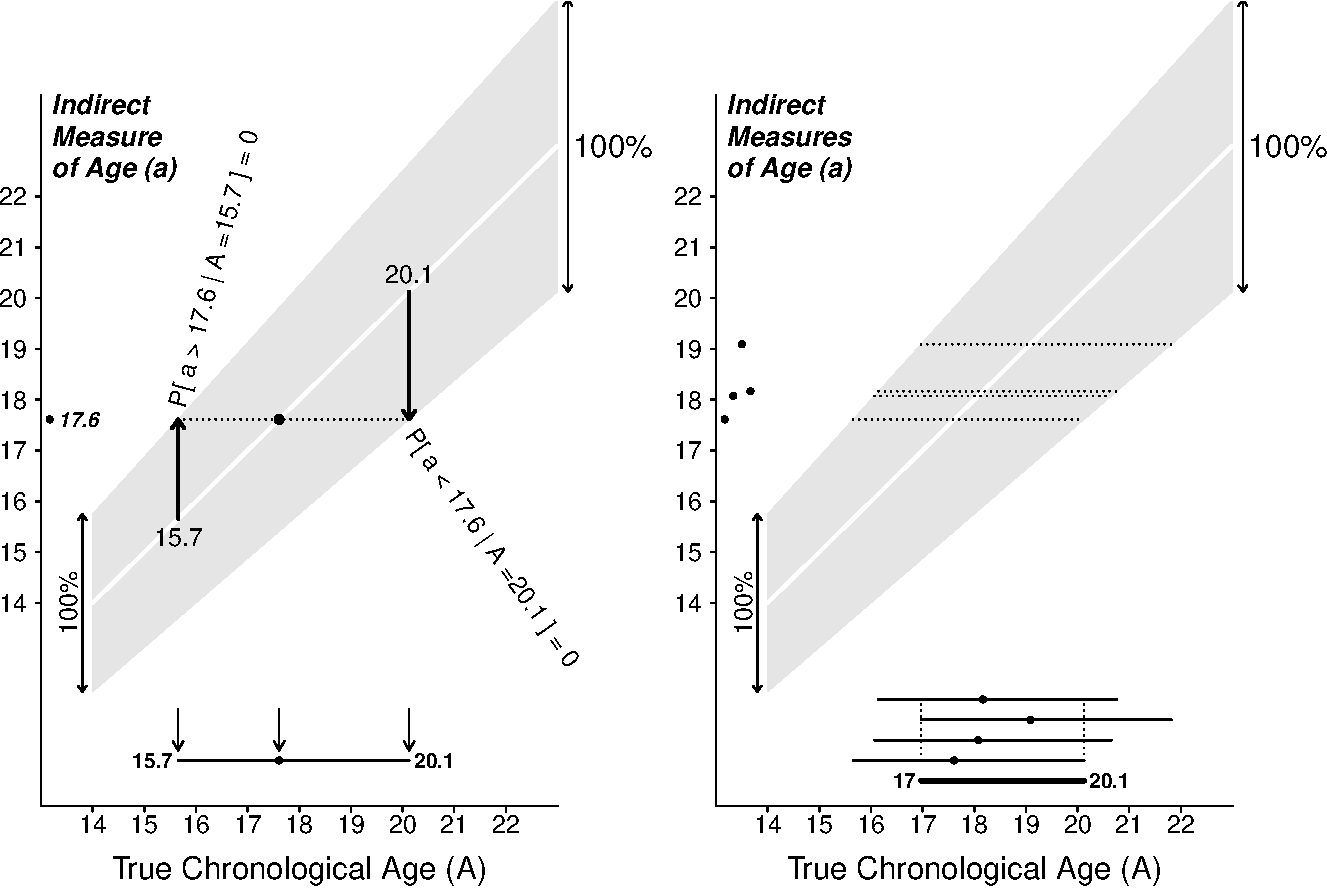
\includegraphics{hanley-ci_files/figure-latex/unnamed-chunk-3-1}

\}

\textbackslash caption\{100\% Confidence Intervals for a person's
chronological age when error distributions (that in this example are
wider at the older ages) are 100\% confined within the shaded ranges.
Left: based on n = 1 measurement; right: based on n = 4 independent
measurements. \}\label{fig:unnamed-chunk-3} \textbackslash end\{figure\}

\textbf{\emph{More data}}

The panel on the right shows how, by obtaining 4 independent
measurements, and finding the interval they have in common, you can
narrow the interval containing the true age.

Can we narrow the interval more, maybe by first averaging the 4
measurements? Should the mean of 4 measurements give us more
information, ie., a tighter interval, that the one based on the overlap?
The sad fact is that, as long we \textbf{insist on 100\% confidence} in
our interval (or our procedure), we can not: the mean of the 3
measurements can still -- theoretically -- be \textbf{anywhere} in the
same 0.75 \(\times\) True Age to 1.25 \(\times\) True Age range -- just
as a single measurement can.

The \textbf{only way to narrow} the interval is to \textbf{take a
chance, cut corners, and accept a lower confidence level}. To do this,
we need to know a bit more about where the pattern (shape) of the error
distribution (**up to now we didn't use the \emph{shape}, just the
\emph{boundaries}). In other words, we need to know how much of the
error distribution is in the corners, so that we can cut them!

In the next section, we will stick for now with Daniel Bernoulli's error
distribution, but cut some corners. (Later on, we will cut some corners
on Laplace's and Gauss's error distributions, but with the same standard
deviation as in Bernoulli's error curve.)

\hypertarget{more-nuanced-intervals}{%
\subsection{More-nuanced intervals}\label{more-nuanced-intervals}}

We will cut 5\% from each corner of the distribution, and focus on the
middlemost 90\%. From the formula for its mathematical shape, we can
calculate that this measurement range is from -1 \(\times\) the radius
of the semi-ellipse to +1 \(\times\) the radius. There is only a 5\%
probability of observing a measurement below (to the left of) this
interval, and a 5\% probability of observing a measurement above (to the
right of) the interval. After we observe our single measurement, we `try
it on' against all possible true-age-scenarios. We retain only those
true-age-scenarios in which the observed measurement would fall within
this central (90\%) range. We discard (`rule out') those age scenarios
in which the measurement would be at one extreme or the other extreme,
in one of the two excluded or `cut' corners.

The left panel shows the (now narrower, and more nuanced) \textbf{range
of true-ages (rahe of parameter values) that is compatible with the
observed measurement of 13.1 years}. In all other age-scenarios, the
13.1 would have been too extreme, and so these scenarios are discarded.
We can think of the \textbf{`ruled in' range} as our (nuanced,
compromise) \textbf{parameter interval}.

Note again the method of constructing this \textbf{non-symmetric}
parameter interval, namely one boundary at a time. It does not fit the
\(\pm\) mold.

It does, however, give a way of talk about such an interval:

\begin{quote}
\textbf{The observed measurement (point-estimate) may be an
underestimate of the parameter: it might have fallen short of the true
parameter value. Or, it may be an underestimate: it might have overshot
the true parameter value. The plus and the minus amounts are the
almost-maximal amounts by which our \emph{shot} might have been
off-target.} (as we will see later, the maximal error can be infinite,
so we have to put some probalistic limits on the error if we are to
narrow the interval).
\end{quote}

Q: Does this \textbf{procedure} for constructing intervals have a 90\%
success rate, if used up and down all of the ages, say from 10 to 30
years? We could try it out with people of known ages. {[}answer by
simulation{]}

You will discover in your simulations that it \textbf{might matter}
whether you simulate the same number of 16 year olds as 10 years, i.e.,
what the \textbf{mix of real ages} is. This does not matter in the 100\%
intervals, but it might if you are more nuanced. For example,instead of
estimating age by an indirect method, pretend you were were
\textbf{estimating a person's height indirectly}, by just
\textbf{measuring their arm span} (at each height, the mean armspan is
very close to the height, but there is a spread of armspans (pardon the
pun!)). And (just like in our example 2 where the spread increases with
the mean) the spread of armspans is larger in people who are 6 feet tall
than it is in people 5 feet tall. BUT, there aren't as many people 5
feet and 6 feet tall as there are people 5 feet 6 inches. So, the
distribution of heights in people with a span of 5 feet 11 might have a
different shape than that in people with a span of 5 feet 6, or 5 feet.
Simulations (or even some diagrams) could settle the issue as to whether
the height-mix (or, in example 2, the age mix) matters. What is your
intuition as to whether it affects the perfornace of your nuanced
parameter estimates? The point is that your method needs to have the
same claimed performance (say 90\%) at any age you throw at it.

\textbackslash begin\{figure\}

\{\centering 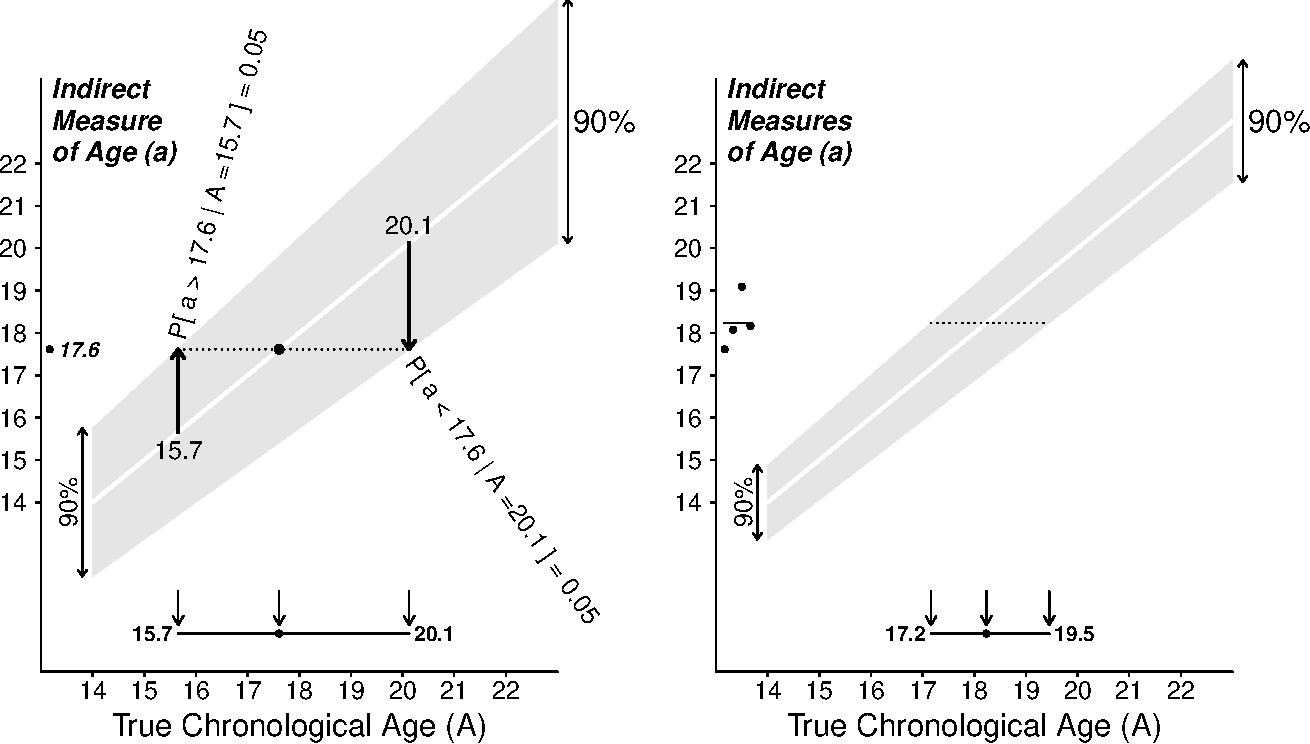
\includegraphics{hanley-ci_files/figure-latex/unnamed-chunk-5-1}

\}

\textbackslash caption\{90\% Confidence intervals for Chronological Age
when only 90\% of the error distributions lie within the shaded
ranges.\}\label{fig:unnamed-chunk-5} \textbackslash end\{figure\}

When we have \(n = 3\) observations (right panel), it is not so easy to
say how confident we should be about the overlap of the 3 intervals.
Instead, we would be bettter off taking the mean of the 3 measurements,
and `trying on' this single mean against the various sampling
distributions of the means of 3 independent measurements from a
semi-circular error distribution. Again, since the range remains the
same, we would again have to cut corners. We will illustrate this when
we now consider the easier-to-work-with Gaussian error distribution.

\textbf{A more realistic error distribution}

Although it makes it easier to demonstrate `100\% confidence' intervals,
Daniel Bernoulli's error distribution is both mathematically unfamiliar,
and a bit unrealistic. And it isn't that easy to see how to use it for
situations where you wiull want to take an average of several
independent indirect measurements. So, we now switch to a more familiar
and more realistic bell-shaped error distribution. It is often called
the Gaussian distribution, even if Gauss was not the first to publish
it. Variations of it were alraedy discovered by deMoivre many decades
earlier, and Gauss' competotor, Laplace , publihed it well before Gauss
did. Gauss claimed he was using it for many years before he published
it. Laplace also used a different (more spiked) error distibution that
today is called after him.

In any case, lets switch to bell-shaped distributions of the age
measurements at each true age, but let's keep the `average squared
deviation' or its square root, the standard deviation, the same as it
was in the Bernoulli model.

on 10 Mark note

NEXT

we deliberately took non-symmetric situations where it is not +/-

Now will show sitations where the error doesnt get bigger of smaller
with the context, and where the `trying-on' is faster.

\hypertarget{summary}{%
\subsection{SUMMARY}\label{summary}}

\begin{itemize}
\item
  what a parameter interval is
\item
  If an error distribution is bounded, we can be 100\% confident in our
  parameter interval, and we can narrow it by taking more measurements.
  Moreover, we don't need to specify the exact shape of the error
  distribution. All that matters are its bounds.
\end{itemize}

I don't think you should take for granted that students (or even
professors!) will know what an error distribution is. So I think a first
point should be to describe what you mean by an error distribution.

\begin{itemize}
\item
  With unbounded error distributions, a 100\% parameter interval may be
  unacceptably wide, even if we take many measurements. Thus, we have to
  `give up something' (in certainty) in order to `get something' (a
  narrower interval). Moreover, we need to either (a) specify a model
  for the shape of the error distribution, or (b) use data-intensive
  techniques, such as re-sampling, to be able to `cut the corners.'
\item
  Either way, a logical way to determine parameter intervals is to have
  them consist of all the parameter-value scenarios in which the
  observed measurement (or summary measurement) is `plausible'. The
  upper limit for the parameter is the scenario in which the measurement
  would be probalistically near the bottom of the corresponding sampling
  distribution; the lower limit is the scenario in which the measurement
  would be near the top of the corresponding sampling distribution.
\item
  If the error (or sampling) distributions have differing spreads at
  different parameter values, then the parameter interval will not be
  symmetric about the point estimate. If the error (or sampling)
  distributions have the same spreads at different parameter values,
  then the parameter interval will be symmetric about the point
  estimate, and thus, easier to calculate.
\end{itemize}

it would be good to give a concrete example here.e.g. repeat the age
example --\textgreater{} It's harder to accurately guess the true age of
someone who is older. perhaps also a good time to mention that in this
situation, the +/- formula will fail you

\begin{itemize}
\tightlist
\item
  It is not correct to view the parameter as `falling' on one or other
  side of the measurement. The true parameter values is fixed, and isn't
  moving or falling anywhere. Rather, it is the observed measurement
  (point-estimate) that may have fallen to the left of (fallen short
  of), and thus provided an underestimate of, the true parameter value:
  Or, it may have overshot the true parameter value, and thus
  overestimated it.
\end{itemize}

This point also explains why the +/- formula fails us

Missing from the above summary points is a direct answer to the question
or criticisms we are likely to face: ``Why do we care about Wilson when
the +/- gives you the same answer?'' The answer to this question is
given indirectly in points 4) and 5). But I think we need to be
explicitly clear about this, since for me at least, is the main
motivation for this chapter.

I also think the objective of the chapter needs to be revised. Based on
our discussions, the point of the chapter is to explain: 1) Why the +/-
formula fails us in the interpretation of a CI and when the spread of
the error distribution is non-constant and 2) Wilson's idea to remedy
the situation.

If you agree with those two objectives, the next question to answer is
how `100\% confidence intervals' and ultimately `cutting corners' helps
you explain the points 1) and 2).

By the way, a simplified version of the Wilson plot you made will be a
great help in visualizing point 3:

\begin{center}\rule{0.5\linewidth}{0.5pt}\end{center}

Another unrealistic feature of our `measurement model' is that the
`error distribution' has a semi-circular (or rather semi-eliptical)
shape. In statistics, it is called the
\href{https://en.wikipedia.org/wiki/Wigner_semicircle_distribution}{`Wigner'
semicircle distribution}. First written about by
\href{http://www.medicine.mcgill.ca/epidemiology/hanley/bios601/Likelihood/Kendall1961OnDanielBernoulliML.pdf}{Daniel
Bernoulli}, predates the error distributions of Laplace and Gauss.

\begin{quote}
\begin{enumerate}
\def\labelenumi{\arabic{enumi}.}
\setcounter{enumi}{4}
\tightlist
\item
  If the \textbf{archer} makes innumerable \textbf{shots}, all with the
  utmost possible care, the arrows will strike sometimes the first band
  next to the mark, sometimes the second, sometimes the third and so on,
  and this is to be understood equally of either side whether left or
  right. Now is it not self-evident that the hits must be assumed to be
  thicker and more numerous on any given band the nearer this is to the
  mark? If all the places on the vertical plane, whatever their distance
  from the mark, were equally liable to be hit, the most skilful shot
  would have no advantage over a blind man. That, however, is the tacit
  assertion of those who use the common rule in estimating the value of
  various discrepant observations, when they treat them all
  indiscriminately. In this way, therefore, the degree of probability of
  any given deviation could be determined to some extent a posteriori,
  since there is no doubt that, for a large number of shots, the
  probability is proportional to the number of shots which hit a band
  situated at a given distance from the mark. Moreover, there is
  \textbf{no doubt that the greatest deviation has its limits which are
  never exceeded} and which indeed are narrowed by the experience and
  skill of the observer. Beyond these limits all probability is zero;
  from the limits towards the mark in the centre the probability
  increases and will be greatest at the mark itself. {[}\textbf{Note}:
  developers and teachers of statistical methods have long made use of
  archery, gunnery, darts, and \textbf{aiming at targets}. Indeed,
  \textbf{the word stochastic}, which refers to randomnees, has its
  roots in the Greek word stokhastikos, meaning able to guess, with the
  root stokhos meaning a target. Klein (1997) writes of `men reasoning
  on the likes of target practice' and describes how this imagery has
  pervaded the thinking and work of natural philosophers and
  \href{http://www.medicine.mcgill.ca/epidemiology/hanley/bios601/Likelihood/letter-jrssa-20110509.pdf}{statisticians}
  {]}
\end{enumerate}
\end{quote}

\begin{quote}
\begin{enumerate}
\def\labelenumi{\arabic{enumi}.}
\setcounter{enumi}{5}
\tightlist
\item
  The foregoing give some idea of a scale of probabilities for all
  deviations, such as each observer should form for himself. It will not
  be absolutely exact, but it will suit the nature of the inquiry well
  enough. The mark set up is, as it were, the centre of forces to which
  the observers are drawn; but these efforts are opposed by innumerable
  imperfections and other tiny hidden obstacles which may produce in the
  observations small chance errors. Some of these will be in the same
  direction and will be cumulative, others will cancel out, according as
  the observer is more or less lucky. From this it may be understood
  that there is some relation between the errors which occur and the
  actual true position of the centre of forces; for another position of
  the mark the outcome of chance would be estimated differently. So we
  arrive at the particular problem of determining the most probable
  position of the mark from a knowledge of the positions of some of the
  hits. It follows from what we have adduced that one should think above
  all of a scale (scala) between the various distances from the centre
  of forces and the corresponding probabilities. Vague as is the
  determination of this scale, it seems to be subject to various axioms
  which we have only to satisfy to be in a better case than if we
  suppose every deviation, whatever its magnitude, to occur with equal
  ease and therefore to have equal probability. Let us suppose a
  straight line in which there are disposed various points, which
  indicate of course the results of different observations. Let there be
  marked on this line some intermediate point which is taken as the true
  position to be determined. Let perpendiculars expressing the
  probability appropriate to a given point be erected. If now a curve is
  drawn through the ends of the several perpendiculars this will be the
  scale of the probabilities of which we are speaking.
\end{enumerate}
\end{quote}

\begin{quote}
\begin{enumerate}
\def\labelenumi{\arabic{enumi}.}
\setcounter{enumi}{6}
\tightlist
\item
  If this is accepted, I think the following assumptions about the scale
  of probabilities can hardly be denied.
\end{enumerate}

\begin{enumerate}
\def\labelenumi{(\alph{enumi})}
\tightlist
\item
  Inasmuch as deviations from the true intermediate point are equally
  easy in both directions, the scale will have two perfectly similar and
  equal branches.
\item
  Observations will certainly be more numerous and indeed more probable
  near to the centre of forces; at the same time they will be less
  numerous in proportion to their distance from that centre. The scale
  therefore on both sides approaches the straight line on which we
  supposed the observed points to be placed.
\item
  The degree of probability will be greatest in the middle where we
  suppose the centre of forces to be located, and the tangent to the
  scale for this point will be parallel to the aforesaid straight line.
\item
  If it is true, as I suppose, that even the least-favoured observations
  have their limits, best fixed by the observer himself, it follows that
  the scale, if correctly arranged, will meet the line of the
  observations at the limits themselves. For at both extremes all
  probability vanishes and a greater error is impossible.
\item
  Finally, the maximum deviations on either side are reckoned to be a
  sort of boundary between what can happen and what cannot. The last
  part, therefore, of the scale, on either side, should approach steeply
  the line on which the observations are sited, and the tangents at the
  extreme points will be almost perpendicular to that line. The scale
  itself will thus indicate that it is scarcely possible to pass beyond
  the supposed limits. Not that this condition should be applied in all
  its rigour if, that is, one does not fix the limits of error
  over-dogmatically.
\end{enumerate}
\end{quote}

\begin{quote}
\begin{enumerate}
\def\labelenumi{\arabic{enumi}.}
\setcounter{enumi}{7}
\tightlist
\item
  If we now construct a \textbf{semi-ellipse} of any parameter on the
  line representing the whole field of possible deviations as its axis,
  this will certainly satisfy the foregoing conditions quite well. The
  parameter {[}radius{]} of the ellipse is arbitrary, since we are
  concerned only with the proportion between the probabilities of any
  given deviation. However elongated or com-pressed the ellipse may be,
  provided it is constructed on the same axis, it will perform the same
  function; which shows that we have no reason to be anxious about an
  accurate description of the scale. In fact we can even use a circle,
  not because it is proved to be the true scale by mathematical
  reasoning, but because it is nearer the truth than an infinite
  straight line parallel to the axis, which supposes that the several
  observations are of equal weight and probability, however distant from
  the true position. This circular scale also lends itself best to
  numerical calculations; meanwhile it is worth observing in advance
  that both hypotheses come to the same whenever the several
  observations are considered to be infinitely small. They also agree if
  the radius of the auxiliary circle is supposed to be infinitely large,
  as if no limits were set to the deviations. Thus if the deviation of
  an observation from the true position is thought of as the sine of a
  circular arc, the probability of that observation will be the cosine
  of the same arc. Let the auxiliary semicircle, which I have just
  described, be called the controlling semicircle (moderator). Where the
  centre of this semicircle is located, the true position, which fits
  the observations best, is to be fixed. Admittedly our hypothesis is,
  to some extent, precarious, but it is certainly to be preferred to the
  common one, and will not be hazardous to those who understand it,
  since the result that they will arrive at will always have a higher
  probability than if they had adhered to the common method. When by the
  nature of the case a certain decision cannot be reached, there is no
  other course than to prefer the more probable to the less probable.
\end{enumerate}
\end{quote}

\begin{quote}
\begin{enumerate}
\def\labelenumi{\arabic{enumi}.}
\setcounter{enumi}{8}
\tightlist
\item
  I will illustrate this line of argument by a trivial example. The
  particular problem is the reconciliation of discrepant observations;
  it is therefore a question of difference of observations. Now if a
  dice-thrower makes three throws with one die so that the second
  exceeds the first by one and the third exceeds the second by two, the
  throws may arise in three ways, viz.~1,2,4 or 2,3,5 or 3,4,6. None of
  these throws is to be preferred to the other two, for each is in
  itself equally probable. If you prefer the one in the middle,
  viz.~2,3,5, the preference is illogical. The same sort of thing
  happens if you choose to consider observations which, so far as you
  are concerned, are accidental, whether they are astronomical or of
  some other kind, as equally probable. Now suppose the thrower produces
  the same result by throwing a pair of dice three times. There will
  then be eight different ways in which he would obtain this result,
  viz.~2,3,5; 3,4,6; 4,5,7; 5,6,8; 6,7,9; 7,8,10; 8,9,11 and 9,10,12.
  But they are far from being all equally probable. It is well known
  that the respective probabilities are proportional to the numbers 8,
  30, 72, 100, 120, 80, 40 and 12. From this known scale I have better
  right to conclude that the fifth set has happened than that any other
  has, because it has the highest probability; and so the three throws
  of a pair of dice will have been 6, 7 and 9. No-one, however, will
  deny that the first set 2, 3 and 5 might possibly have happened, even
  though it has only a fifteenth part of the probability corresponding
  to the fifth set. Forced to choose, I simply choose what is most
  probable. Although this example does not quite square with our
  argument, it makes clear what contribution the investigation of
  probabilities can make to the determination of cases. Now I will come
  more to grips with the actual problem.
\end{enumerate}
\end{quote}

\begin{quote}
\begin{enumerate}
\def\labelenumi{\arabic{enumi}.}
\setcounter{enumi}{9}
\tightlist
\item
  First of all, \textbf{I would have every observer ponder thoroughly in
  his own mind and judge what is the greatest error which he is morally
  certain (though he should call down the wrath of heaven) he will never
  exceed however often he repeats the observation}. He must be his own
  judge of his dexterity and not err on the side of severity or
  indulgence. Not that it matters very much whether the judgement he
  passes in this matter is fitting or somewhat flighty. Then let him
  \textbf{make the radius of the controlling circle equal to the
  aforementioned greatest error}; let this radius be r and hence the
  width of the whole doubtful field = 2r. If you desire a rule on this
  matter common to all observers, I recommend you to suit your judgement
  to the actual observations that you have made: if you double the
  distance between the two extreme observations, you can use it, I
  think, safely enough as the diameter of the controlling circle, or,
  what comes to the same thing, if you make the radius equal to the
  difference between the two extreme observations. Indeed, it will be
  sufficient to increase this difference by half to form the diameter of
  the circle if several observations have been made; my own practice is
  to double it for three or four observations, and .to increase it by
  half for more. Lest this uncertainty offend any one, it is as well to
  note that if we were to make our controlling semicircle infinite we
  should then coincide with the generally accepted rule of the
  arithmetical mean; but if we were to diminish the circle as much as
  possible without contradiction, we should obtain the mean between the
  two extreme observations, which as a rule for several observations I
  have found to be less often wrong than I thought before I investigated
  the matter.
\end{enumerate}
\end{quote}

We must wonder whether its was that this eminent mathematician (who
also, incidentally contributed to the epidemiological debate about
smallpox vaccination) was unable to think of a formula for an error
distribution that did not end abruptly, and that would instead `flow
out' further in both directions. Or was it that he wasn't bothered by
having to find the roots of 5th degree polynomials to find the best
`centre' of his semicircukar distribution? As it turns out, the
mathematics involved in finding (what we now call today) the Maximun
Likelihood Estimator for Laplace's and Gauss's (infinitely wide) error
distributions is much simpler. But the, we have the benefit of
hindsight.

The \textbf{key ideas -- the semi-ellipse and the fixed (assumed known)
-- are highlighted}.

\end{document}
